\documentclass{bmstu}
\usepackage[]{svg}
\usepackage[]{pdfpages}
\usepackage{multirow}
\usepackage{amsmath}
\usepackage{graphicx}

\newcounter{myfigure}
\pretocmd{\figure}{\stepcounter{myfigure}}{}{}
\renewcommand{\thefigure}{\arabic{myfigure}}
\newcounter{mytable}
\pretocmd{\table}{\stepcounter{mytable}}{}{}
\renewcommand{\thetable}{\arabic{mytable}}

\renewcommand{\theequation}{\arabic{equation}}

\setenumerate[1]{label={ \arabic*)}}
\NewBibliographyString{accessmode}
\DeclareFieldFormat{url}{\bibstring{accessmode}\addcolon\space\url{#1}}
\DeclareFieldFormat{title}{#1}
\DefineBibliographyStrings{russian}{
accessmode={Режим доступа:},
urlseen={дата обращения:}
}
\captionsetup[table]{justification=raggedright,singlelinecheck=off}
\renewcommand\labelitemi{---}

\bibliography{biblio}

\begin{document}
\renewcommand{\thelstlisting}{\arabic{lstlisting}}

\makecourseworktitle
    {Информатика и системы управления}
    {Программное обеспечение ЭВМ и информационные технологии}
    {Проектирование программно-аппаратного комплекса <<Куб для визуализации трехмерного изображения>>}
    {Шпаковский~П.~А./ИУ7-53Б}
    {Строганов~Ю.~В.}
    {}

\maketableofcontents

\chapter*{Введение}
\addcontentsline{toc}{chapter}{ВВЕДЕНИЕ}

Компьютерная графика -- это область информационных технологий, которая занимается созданием, обработкой, анализом и визуализацией графических объектов и изображений с использованием компьютерных методов и алгоритмов. 
Она имеет широкий спектр применений, включая развлечения, образование, научные исследования, медицинскую диагностику, архитектурное проектирование, визуализацию данных и многое другое.

Основные задачи, которые решает компьютерная графика.
\begin{enumerate}[label={\arabic*)}]
	\item Создание и редактирование изображений. 
    Компьютерная графика позволяет создавать и редактировать графические объекты и изображения на компьютере. 
    Это включает в себя рисование, моделирование форм и текстур, создание анимаций и спецэффектов.
    \item Визуализация данных. 
    В компьютерной графике данные могут быть представлены в визуальной форме, что делает их более понятными и удобными для анализа. 
    Например, диаграммы, графики и трехмерная визуализация данных используются для отображения статистических и научных результатов.
    \item 3D-моделирование и анимация. 
    Компьютерная графика позволяет создавать трехмерные модели объектов и сцен, а также анимировать их движение и поведение. 
    Это широко используется в фильмах, видеоиграх, архитектурном проектировании и медицинской визуализации.
\end{enumerate}

Общим для всех этих задач является использование математических алгоритмов, программного обеспечения и аппаратных средств для создания, модификации и визуализации графических данных с целью достижения определенных визуальных и функциональных результатов.

Для визуализации трехмерных сцен на конкретной аппаратной платформе часто требуется разрабатывать индивидуальные программные решения, учитывающие особенности данного обеспечения.

Цель данной работы -- спроектировать программно-аппаратный комплекс для построения моделей трехмерных объектов с использованием микроконтроллера, а также разработать макет устройства с шестью гранями, где  каждая грань -- экран, на котором отображается проекция выбранной пользователем трехмерной модели.

Чтобы достичь поставленной цели, требуется решить следующие задачи: 
\begin{itemize}
    \item описать структуру трехмерной сцены, включая объекты, из которых состоит сцена, и определить формат задания исходных данных;
    \item выбрать наиболее подходящий из существующих алгоритмов трехмерной графики, позволяющих синтезировать изображение трехмерной сцены;
    \item реализовать выбранные алгоритмы построения трехмерной сцены;
    \item исследовать возможности микроконтроллеров в области визуализации трехмерной графики.
\end{itemize}

\chapter{Аналитическая часть}

В данной части проводится анализ объектов сцены и существующих алгоритмов построения изображений и выбор более подходящих алгоритмов для дальнейшего использования.

\section{Описание объектов визуализируемой сцены}

Трехмерная сцена состоит из нескольких компонентов.
\begin{enumerate}
    \item Объекты сцены, представляющих из себя многогранники, расположенные в пространстве сцены. 
    Каждый многогранник задается списком полигонов, где полигон описывается множеством точек в трехмерном пространстве.
    \item Материалы и свойства объектов сцены. 
    Каждый объект может иметь определенные свойства, включая цвет, текстуры, прозрачность, отражение и блеск. 
    Эти свойства могут быть формализованы с помощью числовых параметров, которые определяют, как объект взаимодействует со светом и как он будет визуализирован. 
    \item Источники света, которые могут быть формализованы как направленные вектора.
    \item Камера, через которую наблюдается данная сцена. 
    Ее параметры могут включать положение, ориентацию, угол обзора и другие характеристики.
\end{enumerate}

\section{Анализ алгоритмов удаления невидимых линий и поверхностей}

В процессе создания реалистичных изображений ключевой задачей является обеспечение видимости объектов и их частей, учитывая перекрытия между ними. Другими словами, необходимо определить, какие элементы сцены должны быть видны, а какие скрыты от наблюдателя. Эта задача решается с помощью двух групп алгоритмов~\cite{rogers}.
\begin{enumerate}
    \item Алгоритмы, оперирующие в объектном пространстве. 
    Эти алгоритмы связаны с мировой или физической системой координат. 
    Они предназначены для определения видимости объектов, учитывая их пространственное расположение. 
    Однако такие методы требуют значительных вычислительных ресурсов, которые зависят от сложности сцены и необходимой точности. 
    Примерами таких алгоритмов могут быть алгоритм Робертса, алгоритмы на основе списков приоритетов и др.
    \item Алгоритмы, оперирующие в пространстве изображения. 
    Эти алгоритмы ориентированы на систему координат экрана или плоскости изображения, на которую проецируются объекты. 
    Этот подход требует меньше вычислительных ресурсов по сравнению с первой группой, и его объем зависит от разрешения экрана и количества объектов на сцене. 
    Примерами таких алгоритмов являются алгоритм Варнака, алгоритм Z-буфера и метод трассировки лучей.
\end{enumerate}

\subsection{Алгоритм Робертса}

Алгоритм Робертса — это метод удаления невидимых линий и поверхностей в компьютерной графике, который действует в объектном пространстве~\cite{rogers}. 
Его основной целью является определение, какие линии (рёбра) объектов на сцене будут видны из точки наблюдения, а какие будут скрыты за другими объектами.

Алгоритм Робертса делится на 3 этапа.
\begin{enumerate}
    \item На первом этапе каждое тело анализируется индивидуально с целью удаления нелицевых плоскостей. 
    Для каждого тела и каждой грани тела вычисляется уравнение плоскости. 
    После чего проверяется знак уравнения плоскости и формируется матрица тела. 
    \item Удаление из каждого тела тех ребер, которые экранируются всеми остальными телами в сцене. 
    Если задано только одно тело, то алгоритм завершается.
    \item На третьем этапе вычисляются отрезки, которые образуют новые ребра при протыкании телами друг друга. 
\end{enumerate}

За счет того, что алгоритм Робертса работает в объектном пространстве, получается достичь высокую точность результирующего изображения. 
Однако в данном алгоритме используется много трудоемких математических вычислений и сложность растет как квадрат числа объектов на сцене.

\subsection{Алгоритм, использующий Z-буфер}

Алгоритм, использующий Z-буфер, представляет собой один из наиболее простых и широко применяемых методов для удаления невидимых поверхностей. Этот алгоритм оперирует в пространстве изображения и основывается на идее использования двух буферов: буфера кадра и Z-буфера.

\begin{enumerate}
    \item Буфер кадра (англ. Frame Buffer). 
    Этот буфер представляет собой массив пикселей, в котором будут храниться атрибуты (например, цвет) каждого пикселя на экране.
    \item Z-буфер (англ. Depth Buffer). 
    Это отдельный буфер глубины, который будет хранить глубину (Z-координату) каждого пикселя на экране. 
    Исходно он заполняется максимально возможными значениями глубины.
\end{enumerate}

Алгоритм работает следующим образом.
\begin{enumerate}
    \item Перед началом работы буфер кадра заполняется информацией о фоновом изображении, а Z-буфер заполняется минимальными значениями глубины.
    \item Для каждого объекта на сцене: 
    \begin{itemize}
        \item полигоны объекта преобразуются в растровую форму;
        \item для каждого пикселя текущего полигона проверяется его Z-координата (глубина) в сравнении с соответствующим значением в Z-буфере;
        \item если Z-координата текущего пикселя меньше, чем значение в Z-буфере, то пиксель заносится в буфер кадра, а его Z-координата обновляется в Z-буфере.
    \end{itemize}
    \item На выходе получается изображение, в котором каждый пиксель находится в буфере кадра в соответствии с его видимостью и глубиной.
\end{enumerate}

К преимуществам относятся простота реализации, которая позволяет достичь хороших результатов без сложной сортировки объектов. Также алгоритм эффективно обрабатывает сцены с большим количеством объектов.

К недостаткам можно отнести потребление большого объема памяти для хранения двух буферов, а также могут быть проблемы с прозрачностью и лестничным эффектом (ступенчатость на границах объектов).

\subsection{Алгоритм Варнока}

Алгоритм Варнока -- это метод удаления невидимых поверхностей в компьютерной графике, который использует разбиение сцены на более мелкие части для определения видимости объектов. 
Алгоритм работает в пространстве изображения и анализирует область на экране дисплея (окно) на наличие в них видимых элементов~\cite{delinvis}. 

Идея алгоритма Варнока заключается в разбиении экрана на рекурсивные прямоугольники, которые обозначают различные части сцены. 
Затем каждый прямоугольник проверяется на наличие видимых объектов. 
Если внутри прямоугольника объекты видимы, он разбивается на более мелкие прямоугольники, и процесс продолжается до достижения требуемого уровня детализации или пока не будут найдены видимые объекты.

Процесс алгоритма Варнока.
\begin{enumerate}
    \item Разбиение экрана. 
    Исходный экран разбивается на начальные прямоугольники. 
    Эти прямоугольники могут представлять собой целый экран или другие крупные области.
    \item Проверка видимости. 
    Для каждого прямоугольника выполняется проверка видимости объектов, находящихся внутри него. 
    \includeimage
        {relationship}
        {f}
        {h}
        {0.8\textwidth}
        {Варианты взаимного расположения многоугольников~\cite{delinvis}}
    \item Принятие решения. 
    В зависимости от результата проверки видимости объектов внутри прямоугольника, он может быть разбит на более мелкие подпрямоугольники или объединен с другими прямоугольниками. 
    Этот процесс продолжается рекурсивно.
    \item Заполнение буфера кадра. 
    Для видимых прямоугольников или их частей выполняется заполнение буфера кадра атрибутами объектов.
    \item Завершение. 
    Процесс рекурсивного разбиения и проверки видимости продолжается до достижения требуемого уровня детализации или до тех пор, пока не будет достигнута наименьшая обрабатываемая единица.
\end{enumerate}

Преимущества алгоритма Варнока включают возможность обработки сложных сцен, включая объекты с перекрывающимися поверхностями. 
Однако он может потребовать больших вычислительных ресурсов и времени, особенно при работе с детализированными сценами. 

\subsection{Алгоритм, использующий список приоритетов}

Этот алгоритм базируется на упорядочивании объектов сцены в зависимости от их приоритета, который определяется их удаленностью от наблюдателя или глубиной в сцене. 
Идея заключается в начальном рендеринге объектов, находящихся на большем расстоянии от наблюдателя, и последующем перекрытии их ближайшими объектами.

Сначала происходит сортировка объектов по глубине, что создает первоначальный список приоритетов. 
Затем этот список подвергается коррекции через выполнение тестов на экранирование для каждой пары многоугольников в списке. 
Эти тесты могут быть достаточно затратными по времени и сложности реализации. 
Суть тестов заключается в определении, перекрывает ли один многоугольник другой, и, если да, то какой из них ближе к наблюдателю.

Важно отметить, что идентификация случаев пересечения и циклического перекрытия многоугольников в этом алгоритме является сложной задачей. 
Вследствие этого алгоритм может сталкиваться с ограничениями в эффективности и точности при обработке таких сцен, где объекты перекрывают друг друга в сложных сценариях.

\subsection{Алгоритм трассировки лучей}

Алгоритм трассировки лучей -- это метод удаления невидимых поверхностей в компьютерной графике, который симулирует путь световых лучей, падающих на объекты в сцене. 
Он создает фотореалистичные изображения, учитывая отражение, преломление и тени. 

Предполагается, что наблюдатель находится на бесконечности положительной полуоси Z, и все световые лучи от наблюдателя параллельны этой оси. 
В ходе алгоритма обратной трассировки лучей, начиная от наблюдателя, генерируются лучи и находятся пересечения этих лучей с объектами сцены. 
Путем анализа этих пересечений определяется самая ближняя точка пересечения по оси Z, которая представляет видимую часть поверхности. 
Атрибуты этого объекта затем используются для определения характеристик пикселя, через который проходит этот световой луч.

Для создания реалистичных эффектов освещения алгоритм генерирует дополнительные лучи от точек пересечения к источникам света. 
Если на пути такого луча встречается непрозрачный объект, это означает, что данная точка находится в тени.

\includeimage
    {ray_tracing}
    {f}
    {h}
    {1.0\textwidth}
    {Визуализация алгоритма трассировки лучей~\cite{tracing}}

Основными преимуществами данного алгоритма являются реалистичность получаемого изображения и возможность анализировать наложение света. 
Однако из-за использования большого количества лучей производительность алгоритм снижается, поскольку для каждого луча необходимо производить поиск пересечений с объектами сцены.

\section{Анализ алгоритмов закраски}

\subsection{Простая закраска}
Применяется закрашивание, в котором каждая грань получает один уровень интенсивности, вычисляемый согласно закону Ламберта. 
В результате такой закраски все плоские поверхности, включая те, что аппроксимируют фигуры, подвергаются однородному окрашиванию. 
В случае фигур вращения это может вызвать появление ложных границ между поверхностями.

Этот метод обладает высокой производительностью, однако все пиксели на грани получают одинаковую интенсивность, что придает сцене нереалистичный вид. 
Несмотря на это, метод очень прост в реализации и не требует значительных вычислительных ресурсов.

\subsection{Закраска по Гуро}

Закраска по методу Гуро основана на билинейной интерполяции интенсивностей на поверхности грани. 
Этот метод создает иллюзию плавной криволинейной поверхности, так как интенсивность вычисляется для каждой точки грани, что способствует мягкому переходу между цветами.

Закраска по методу Гуро хорошо сочетается с простой моделью освещения, основанной на диффузном отражении света. 
Она значительно улучшает качество изображения, придавая ему более реалистичный вид.

% Вопрос про ГОСТ, 2 элемента списка
Однако у этого метода есть свои недостатки:
\begin{itemize}
    \item возникает эффект полос Маха -- артефакт, проявляющийся в виде полос вдоль граней изображения;
    \item из-за сглаживания интенсивностей может быть утрачена четкая граница между гранями многогранника, что в некоторых ситуациях может привести к неверному визуальному результату.
\end{itemize}

Процедура закрашивания граней методом Гуро состоит из четырех последовательных этапов.
\begin{enumerate}
    \item Вычисление граничных нормалей. 
    На этом этапе определяются нормали для каждой отдельной грани. 
    Нормаль -- это вектор, перпендикулярный к поверхности грани и указывающий направление в пространстве.
    \item Определение вершинных нормалей. 
    Затем определяются нормали в вершинах объекта. 
    Нормаль в вершине вычисляется как среднее значение нормалей граней, смежных с данной вершиной. 
    Это позволяет создать плавные переходы между нормалями граней и учесть геометрическую структуру объекта.
    \item Вычисление яркостей в вершинах. 
    Исходя из нормалей в вершинах, определяются значения яркостей (интенсивностей) в этих вершинах, согласно выбранной модели отражения света. 
    Это позволяет учесть, как свет падает на разные части объекта.
    \item Закрашивание граней. 
    Наконец, происходит закрашивание полигонов граней. 
    Каждая грань получает цвет, который вычисляется путем линейной интерполяции значений интенсивностей в вершинах этой грани. 
    Это создает плавные переходы цветов на поверхности и добавляет визуальную реалистичность объекту.
\end{enumerate}

\subsection{Закраска по Фонгу}

Закраска по модели Фонга, по своей концепции, схожа с закраской по методу Гуро, но имеет отличие в том, как интерполируются значения. 
В методе Гуро производится интерполяция значений интенсивности для всех точек полигона, тогда как в методе Фонга интерполируются векторы нормалей граней, и на основе этих нормалей определяется интенсивность для каждой точки~\cite{phong}.

Этапы алгоритма закраски по Фонгу следующие.
\begin{enumerate}
    \item Вычисление нормалей для каждой грани.
    \item На основе нормалей граней определяются нормали в вершинах. 
    В каждой точке грани интерполируется вектор нормали, учитывая соседние вершины.
    \item С использованием направления векторов нормали определяется цвет точек грани в соответствии с выбранной моделью освещения.
\end{enumerate}

Алгоритм закраски по модели Фонга требует больше вычислительных ресурсов по сравнению с предыдущими методами, но он позволяет достичь лучшей локальной аппроксимации кривизны поверхности. 
Это приводит к более реалистичному изображению, так как метод учитывает изменения в направлениях нормалей на поверхности, что способствует созданию более точных эффектов освещения.

\section{Критерии выбора алгоритмов трехмерной визуализации}
При выборе алгоритмов компьютерной графики для визуализации трехмерной сцены следует учитывать особенности платформы, с помощью которой будет решаться задача. 
В данном случае необходимо рассмотреть возможности микроконтроллеров.

\begin{enumerate}
    \item Объем оперативной памяти на микроконтроллере достаточно ограничен. 
    Обычно он составляет не больше нескольких мегабайт. 
    Поэтому при выборе алгоритмов стоит учитывать размер используемых структур данных и затраченной памяти в целом.
    \item Вычислительная мощность микроконтроллеров также невысокая, поэтому при выборе алгоритма стоит учитывать его простоту и эффективность работы. 
    Немаловажной будет являться сложность работы алгоритма, по возможности, она должна быть линейной в зависимости от количества объектов сцены. 
    \item Объем встроенной постоянной памяти в микроконтроллерах небольшой и составляет не более 2 мегабайт. 
    Исходя из этого размер исполняемого файла должен быть меньше, поэтому стоит выбирать алгоритмы, реализация которых более лаконичная и компактная.
\end{enumerate}

Для поставленной задачи критерий, связанный с объемом оперативной памяти, будет приоритетным.

\section{Вывод из аналитической части}

Проанализировав алгоритмы удаления невидимых линий и поверхностей и различные алгоритмы закраски, а также рассмотрев критерии выбора наиболее оптимального алгоритма для поставленной задачи визуализации трехмерной сцены с использованием микроконтроллера, можно сделать вывод, что алгоритм Варнока и алгоритм простой закраски подходят лучше всего. 
Алгоритм Варнока использует оптимальное количество памяти и требует меньшей вычислительной мощности, по сравнению с другими алгоритмами. 
Простая закраска наименее ресурсоемкая из всех алгоритмов закраски, при этом позволяет достичь поставленной цели. При выборе алгоритмов ключевую роль играли особенности аппаратной платформы.

\chapter{Конструкторская часть}

\chapter{Технологическая часть}

В данном разделе будут рассмотрены детали реализации программно-аппаратного комплекса, описанного в конструкторской части работы, и приведены примеры работы макета устройства.

\section{Средства реализации}
Для реализации данной курсовой работы выбран язык программирования C++~\cite{cpp-lang}.
Язык предоставляет высокую производительность при использовании в компьютерной графике. Также используются вставки на языке C для работы с низкоуровневым интерфейсом микроконтроллера и обеспечения коммуникации с периферией. Драйвер дисплея с чипом ST7789 в своей реализации использует язык C. 

Для отладки программы используется интерфейс SWD (Serial Wire Debug)~\cite{swd} и программа OpenOCD~\cite{openocd}, предоставляющая возможность удаленной отладки с персонального компьютера. 

Взаимодействие пользователя с программой осуществляется с помощью консоли, которая реализуется за счет протокола UART. Для соединения компьютера и микроконтроллера используется преобразователь UART в USB.

\section{Особенности реализации}

Макет устройства использует два протокола взаимодействия с периферией: SPI и UART. UART применяется для реализации консольного пользовательского интерфейса для взаимодействия с трехмерной сценой. SPI для работы дисплеев.

При конструировании устройства была выявлена проблема, связанная с питанием. Для работы шести дисплеев требуется большая мощность источника питания, по сравнению с той, которая предоставляется микроконтроллером (3.3 В). Для работы макета устройства необходимо использовать стационарный источник питания с напряжением 12 В. В связи с отсутствием такого источника, аппаратный комплекс был переработан и на данный момент количество дисплеев равно двум. Однако в исходный код программы заложена возможность визуализации трехмерной сцены на шести дисплеях. Таким образом, при наличии стационарного источника питания, программно-аппаратный комплекс будет работать корректно. 

\section{Форматы описания трехмерной сцены}
Геометрическое описание объектов сцены представляется в формате Wavefront OBJ~\cite{obj}. В данной работе используется полигональная модель представления трехмерных объектов. Формат obj хранит текстовую информацию о вершинах полигонов, их нормалях и о материале полигона. 

Материал полигона задается в формате Wavefront MTL~\cite{mtl}. В случае использования простой закраски при визуализации сцены необходимо получить из файла только компоненту, задающую цвет полигона. 

Сцена представляет из себя объекты, расположенные в пространстве, камеру и источники освещения. Эти данные представлены в виде текстового файла формата scene. Данный формат схож с форматами obj и mtl.

В листингe \ref{lst:sphere.scene} приведен пример файла описания трехмерной сцены.
\includelisting
    {sphere.scene}
    {Пример файла описания трехмерной сцены}

\section{Модули программы}
Разработанный программный комплекс разбит на следующие модули:
\begin{itemize}
    \item main.cpp -- файл, содержащий точку входа в программу. В нем происходит обработка команд от пользователя и основной цикл визуализации сцены;
    \item loader.cpp -- файл, содержащий функции для загрузки информации об объектах сцены из файлов в форматах obj, mtl, scene;
    \item dataset.cpp -- сгенерированный файл, включающий в себя описания нескольких объектов сцены, которые позже будут скопировны во флеш память микроконтроллера вместе с машинным кодом;
    \item math -- модуль, реализующий математические операции и структуры данных;
    \item render -- модуль, отвечающий за отрисовку трехмерной сцены;
    \item scene -- модуль, описывающий структуры данных для описания сцены;
    \item lib -- сторонние библиотеки, использующиеся в работе;
    \item desktop -- реализация алгоритмов визуализации для персонального компьютера.
\end{itemize}

\section{Реализация алгоритмов визуализации}
В листингe \ref{lst:warnock1.cpp} приведен код реализации алгоритма Варнока удаления невидимых граней.
\pagebreak
\includelisting
    {warnock1.cpp}
    {Листинг кода реализации алгоритма Варнока}
\pagebreak
\includelisting
    {warnock2.cpp}
    {Продолжение листинга кода реализации алгоритма Варнока}

Переданное окно делится на 4 равных части и они заносятся в стек. Данный процесс длится до тех пор, пока объект, попадающий в окно не станет тривиально видимым или тривиально невидимым. Итеративная реализация алгоритм позволяет уменьшить объем используемой памяти.

\subsection{Классический алгоритм Варнока}
В листингe \ref{lst:use1.cpp} приведен код, использующий реализацию классического алгоритма Варнока, без использования аппаратных средств ускорения визуализации. Предварительное разбиение окна на шесть частей не производится.

\pagebreak
\includelisting
    {use1.cpp}
    {Классический алгоритм Варнока}

\subsection{Модифицированный  алгоритм Варнока}
В листингe \ref{lst:use2.cpp} приведен код, использующий реализацию модифицированного алгоритма Варнока, который использует аппаратное ускорение с помощью прямого доступа к памяти. Предварительно окно разбивается на шесть частей для более эффективной пересылки данных по DMA. 
\includelisting
    {use2.cpp}
    {Модифицированный алгоритм Варнока}

\section{Пользовательский интерфейс}
В данной работе был реализован консольный пользовательский интерфейс. Для управления визуализируемой сценой используется набор текстовых команд, каждая из которых принимает ряд аргументов. Пользователь может загрузить новую трехмерную сцену по ее названию или вывести список всех доступных сцен в программе. Также возможно вращение камеры на заданный угол, приближение камеры и ее перемещение. 

Поддерживаются следующие команды:
\begin{itemize}
    \item help -- вывод информации о командах;
    \item models -- вывод списка названий доступных трехмерных сцен;
    \item load <название сцены> -- загрузка сцены по ее названию;
    \item camera set cp <x, y, z> ct <x, y, z> cu <x, y, z> -- установка камеры по трем векторам направлений;
    \item camera rotate <rx, ry, rz> -- вращение камеры, где rx, ry, rz - углы поворота по осям в градусах;
    \item camera scale <k> -- масштабирование камеры, где k - коэффициент масштабирования;
    \item camera reset -- сброс настроек камеры к значению по умолчанию.
\end{itemize}

\section{Пример работы программно-аппаратного комплекса}
На рисунке \ref{img:renderer} представлен пример визуализации трехмерной сцены, включающей две низкополигональные сферы и три источника света.
\includeimage
    {renderer}
    {f}
    {H}
    {1.0\textwidth}
    {Пример работы программно-аппаратного комплекса}

На рисунке \ref{img:interface} представлен пример работы с пользовательским интерфейсом программы.
\includeimage
    {interface}
    {f}
    {H}
    {1.0\textwidth}
    {Пример пользовательского интерфейса}

\section{Вывод из технологической части}
В данном разделе были рассмотрены детали реализации программно-аппаратного комплекса, описанного в конструкторской части работы, и приведены примеры работы макета устройства, а также пример работы с пользовательским интерфейсом.

\chapter{Исследовательская часть}

В данной части будет проводено исследование разработанных алгоритмов компьютерной графики для использования их с применением аппаратных возможностей микроконтроллера. 

Целью исследования является определение зависимости времени выполнения классического и модифицированного алгоритмов Варнока от количества визуализируемых полигонов на сцене, а также сравнение данных алгоритмов. Замеры времени проводятся для количества полигонов, изменяющегося от 50 до 500 с шагом измерения в 50 полигонов. 

\section{Средства реализации}
При проведении исследования используется микроконтроллер RP2040~\cite{rp2040} в плате Raspberry Pi Pico. Для отображения итогового изображения используются два экрана с разрешением 240x240 пикселов, подключенные по одной шине SPI. 

Характеристики микроконтроллера RP2040:
\begin{itemize}
    \item 32-битный процессор ARM Cortex-M0+\~cite{cortex-m0};
    \item тактовая частота процессора -- 133 МГц;
    \item объем оперативной памяти -- 264 Кб;
    \item объем постоянной памяти -- 2 Мб;
    \item частота шины SPI -- 40 МГц;
    \item наличие встроенного контроллера DMA~\cite{dma}. 
\end{itemize}

Для замера времени работы реализованных алгоритмов используется системый системный таймер SysTick~\cite{systick}, который является частью процессоров семейства Cortex-M. 

\section{Результаты исследования}
В таблице \ref{tbl:time} приведены результаты замеров времени для двух реализаций алгоритма Варнока удаление невидимых граней.

\begin{table}[H]
    \caption{\label{tbl:time}Замеры времени сравнения алгоритмов Варнока}
	\resizebox{\textwidth}{!}{
	\def\arraystretch{1.5}
    \begin{tabular}{|c|c|c|}
    \hline
    Кол-во полигонов, шт &
      \begin{tabular}[c]{@{}c@{}}Модифицированный \\ алгоритм Варнока\end{tabular} &
      \begin{tabular}[c]{@{}c@{}}Классический \\ алгоритм Варнока\end{tabular} \\ \hline
    50  & 1452  & 2032  \\ \hline
    100 & 3132  & 4698  \\ \hline
    150 & 5076  & 7360  \\ \hline
    200 & 6349  & 8903  \\ \hline
    250 & 9071  & 12699 \\ \hline
    300 & 10865 & 14124 \\ \hline
    350 & 12168 & 18435 \\ \hline
    400 & 15323 & 22984 \\ \hline
    450 & 17342 & 23744 \\ \hline
    500 & 19891 & 29836 \\ \hline
    \end{tabular}
    }
\end{table}

На рисунке \ref{img:plot} представлен график зависимости времени работы двух алгоритмов Варнока в зависимости от заданного количества полигонов.

\begin{figure}[H]
	\centering
	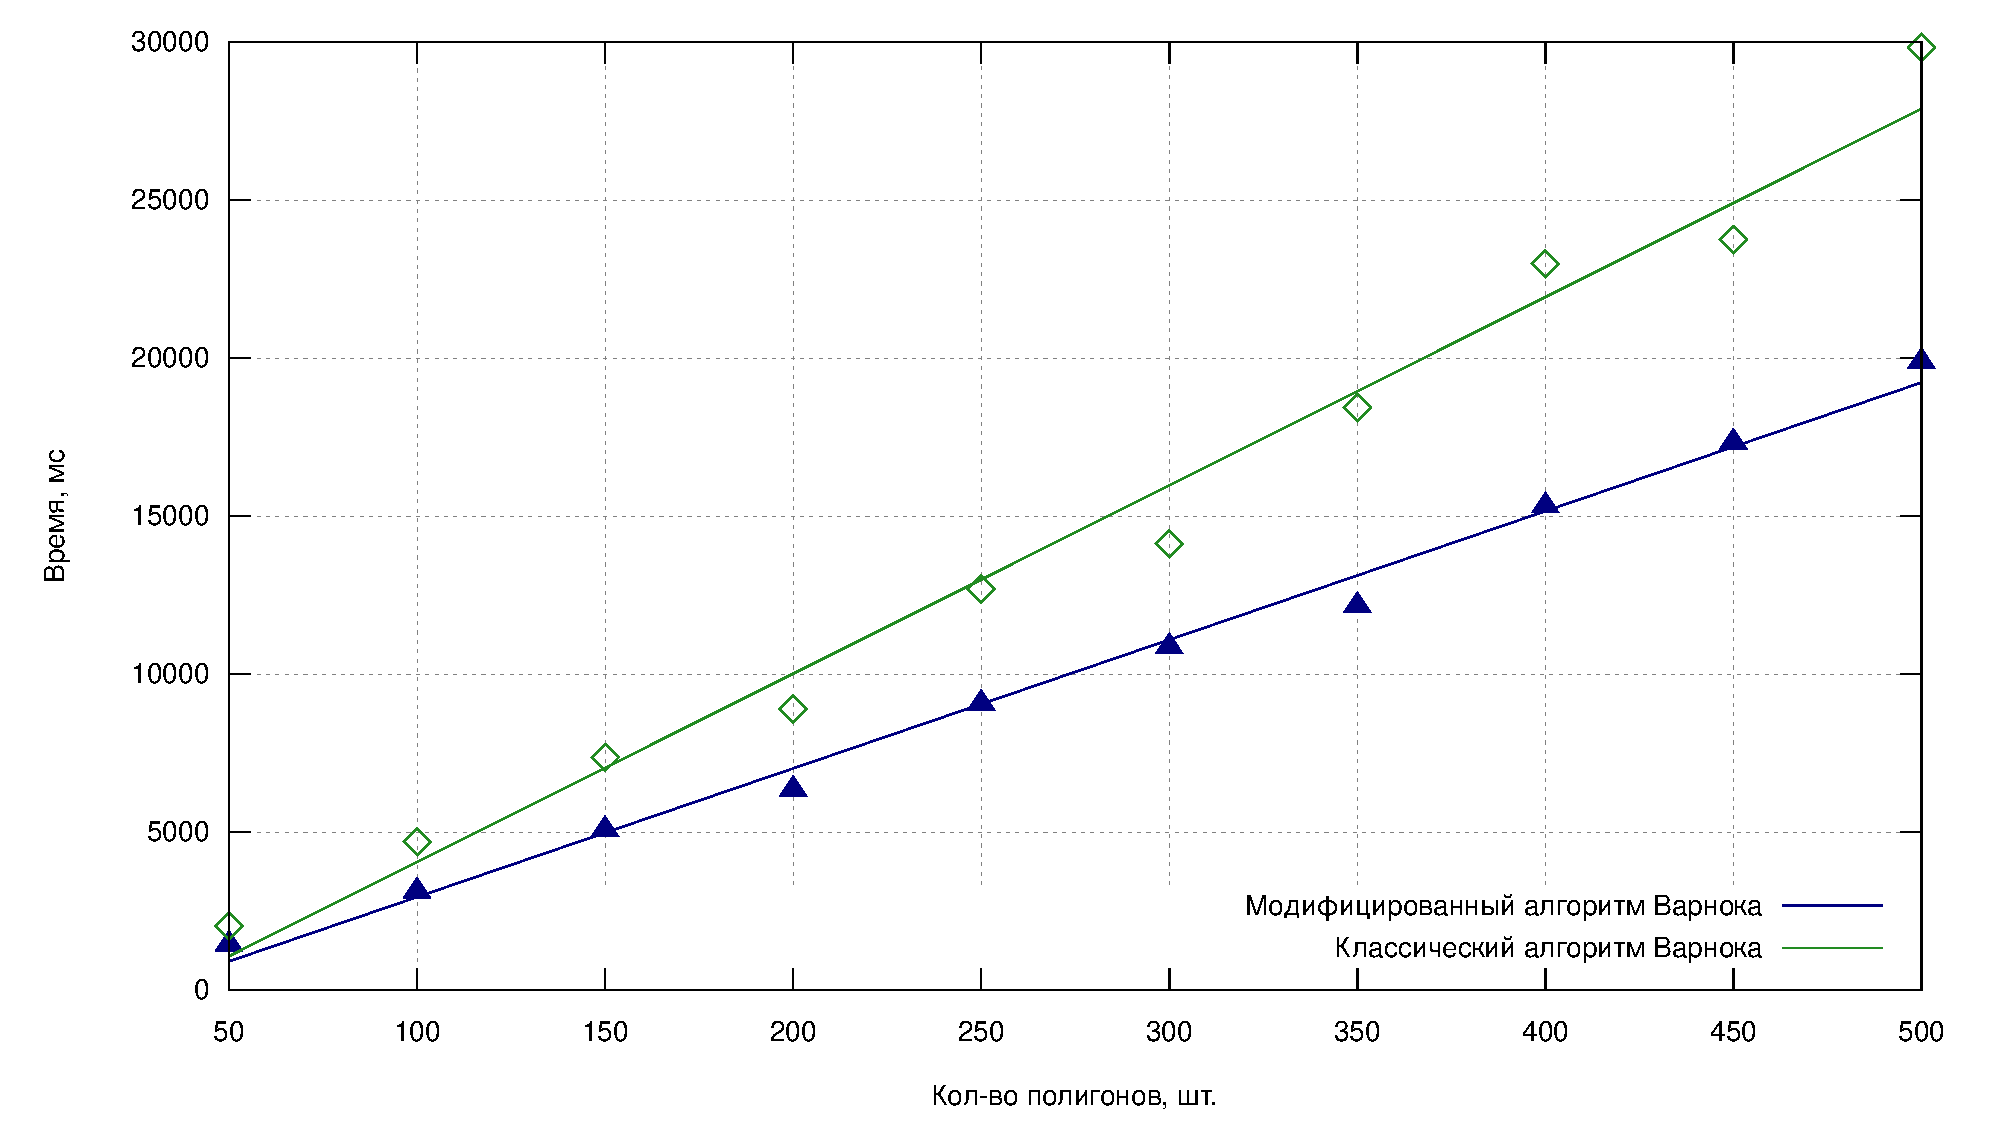
\includegraphics[height=0.35\textheight]{inc/img/plot.pdf}
	\caption{Сравнение классического и модифицированного алгоритмов Варнока}
	\label{img:plot}
\end{figure}

\section{Вывод из исследовательской части}
В результате исследования можно заметить, что модифицированный алгоритм Варнока превосходит классическую реализацию алгоритма по эффективности. Таким образом, за счет использования аппаратных особенностей микроконтроллера удалось достичь меньшего времени визуализации сцены. Прямой доступ к памяти обеспечивает более эффективный доступ к периферии, при этом нагрузка на процессор не увеличивается.

\chapter*{Заключение}
\addcontentsline{toc}{chapter}{ЗАКЛЮЧЕНИЕ}

В ходе выполнения данной курсовой работы были выполнены следующие задачи:
\begin{itemize}
    \item описана структуру трехмерной сцены, включая объекты, из которых состоит сцена, и определен формат задания исходных данных;
    \item выбран наиболее подходящий из существующих алгоритмов трехмерной графики, позволяющих синтезировать изображение трехмерной сцены;
    \item реализованы выбранные алгоритмы построения трехмерной сцены;
    \item исследованы возможности микроконтроллеров в области визуализации трехмерной графики.
\end{itemize}

Однако, в процессе разработки матека устройства были обнаружены некоторые проблемы, описанные в технологической части данной работы. С учетом этого факта, архитектура устройства была переработана. В результате макет устройства включает в себя микроконтроллер и два экрана, задающих две соседние грани куба, на каждой из которых изображается проекция трехмерной сцены.   


\makebibliography

\chapter*{Приложение А}
\addcontentsline{toc}{chapter}{ПРИЛОЖЕНИЕ А}
\section*{Презентация к курсовой работе}


\end{document}
